\documentclass{class}

%-----------------------------------------------------------------
\titleind{Laporan Praktikum}

\fullname{Afrizal Dani Saoqi}

\idnum{17/413500/TK/45940}

\papername {Sistem Tertanam dan IoT}

\degree{Teknik Elektro}

\yearsubmit{2020}

\program{Teknik Elektro}

\dept{Teknik Elektro dan Teknologi Informasi}


%-----------------------------------------------------------------



\usepackage[titles]{tocloft}
\renewcommand\cftfigpresnum{Gambar\  }
\renewcommand\cfttabpresnum{Tabel\   }

%Untuk hyperlink dan table of content
\usepackage{hyperref}
\newlength{\mylenf}
\settowidth{\mylenf}{\cftfigpresnum}
\setlength{\cftfignumwidth}{\dimexpr\mylenf+2em}
\setlength{\cfttabnumwidth}{\dimexpr\mylenf+2em}

%Untuk Bold Face pada Keterangan Gambar
\usepackage[labelfont=bf]{caption}

%Untuk caption dan subcaption
\usepackage{caption}
\usepackage{subcaption}
\usepackage{listings}
\usepackage{xcolor}

\definecolor{codegreen}{rgb}{0,0.6,0}
\definecolor{codegray}{rgb}{0.5,0.5,0.5}
\definecolor{codepurple}{rgb}{0.58,0,0.82}
\definecolor{backcolour}{rgb}{0.95,0.95,0.92}

\lstdefinestyle{mystyle}{
    backgroundcolor=\color{backcolour},   
    commentstyle=\color{codegreen},
    keywordstyle=\color{magenta},
    numberstyle=\tiny\color{codegray},
    stringstyle=\color{codepurple},
    basicstyle=\ttfamily\footnotesize,
    breakatwhitespace=false,         
    breaklines=true,                 
    captionpos=b,                    
    keepspaces=true,                 
    numbers=left,                    
    numbersep=5pt,                  
    showspaces=false,                
    showstringspaces=false,
    showtabs=false,                  
    tabsize=2
}

\lstset{style=mystyle}
\usepackage{rotating}
\begin{document}
\cover
    \chapter{Pengenalan}
    \section{Raspberry Pi}
    Raspberry Pi merupakan SBC \emph{(Single Board computer)} yang dikembangkan oleh Raspberry Pi Foundation.
    Pada praktikum ini saya menggunakan Raspberry Pi 3 Model B. Berikut spesifikasi Raspberry Pi 3B dan Pinout GPIO pada Raspberry Pi 3B. \\
    \begin{table}[h!]
      \begin{tabular}{|c|c|c|c|c|c|c|c|}
          \hline
          $SOC$ & Broadcom BCM2837 \\ \hline
          $CPU$ & ARM Cortex A53 64Bit @1.2GHz \\ \hline
          $GPU$ & VideoCore IV @400MHz\\ \hline
          $RAM$ & 1GB LPDDR2 @900MHz\\ \hline
          $Ethernet$ & 10/100Mbps Ethernet\\ \hline
          $Wifi$ & 2.4GHz IEEE 802.11n\\ \hline
          $Bluetooth$ & Bluetooth 4.1 Classic, Bluetooth Low Energy.\\ \hline
          $Storage$ & MicroSD\\ \hline
          $GPIO$ & 40-pin header\\ \hline
          $Max Power$ & 2.5A @5V\\ \hline
          $Ports$ & 4x 2.0 USB Port\\ \hline
          $Video Output$ & 1x HDMI\\ \hline
      \end{tabular}
      \caption{Spesifikasi Raspberry Pi 3B}
  \end{table}
  \begin{figure}[H]
    \centering
        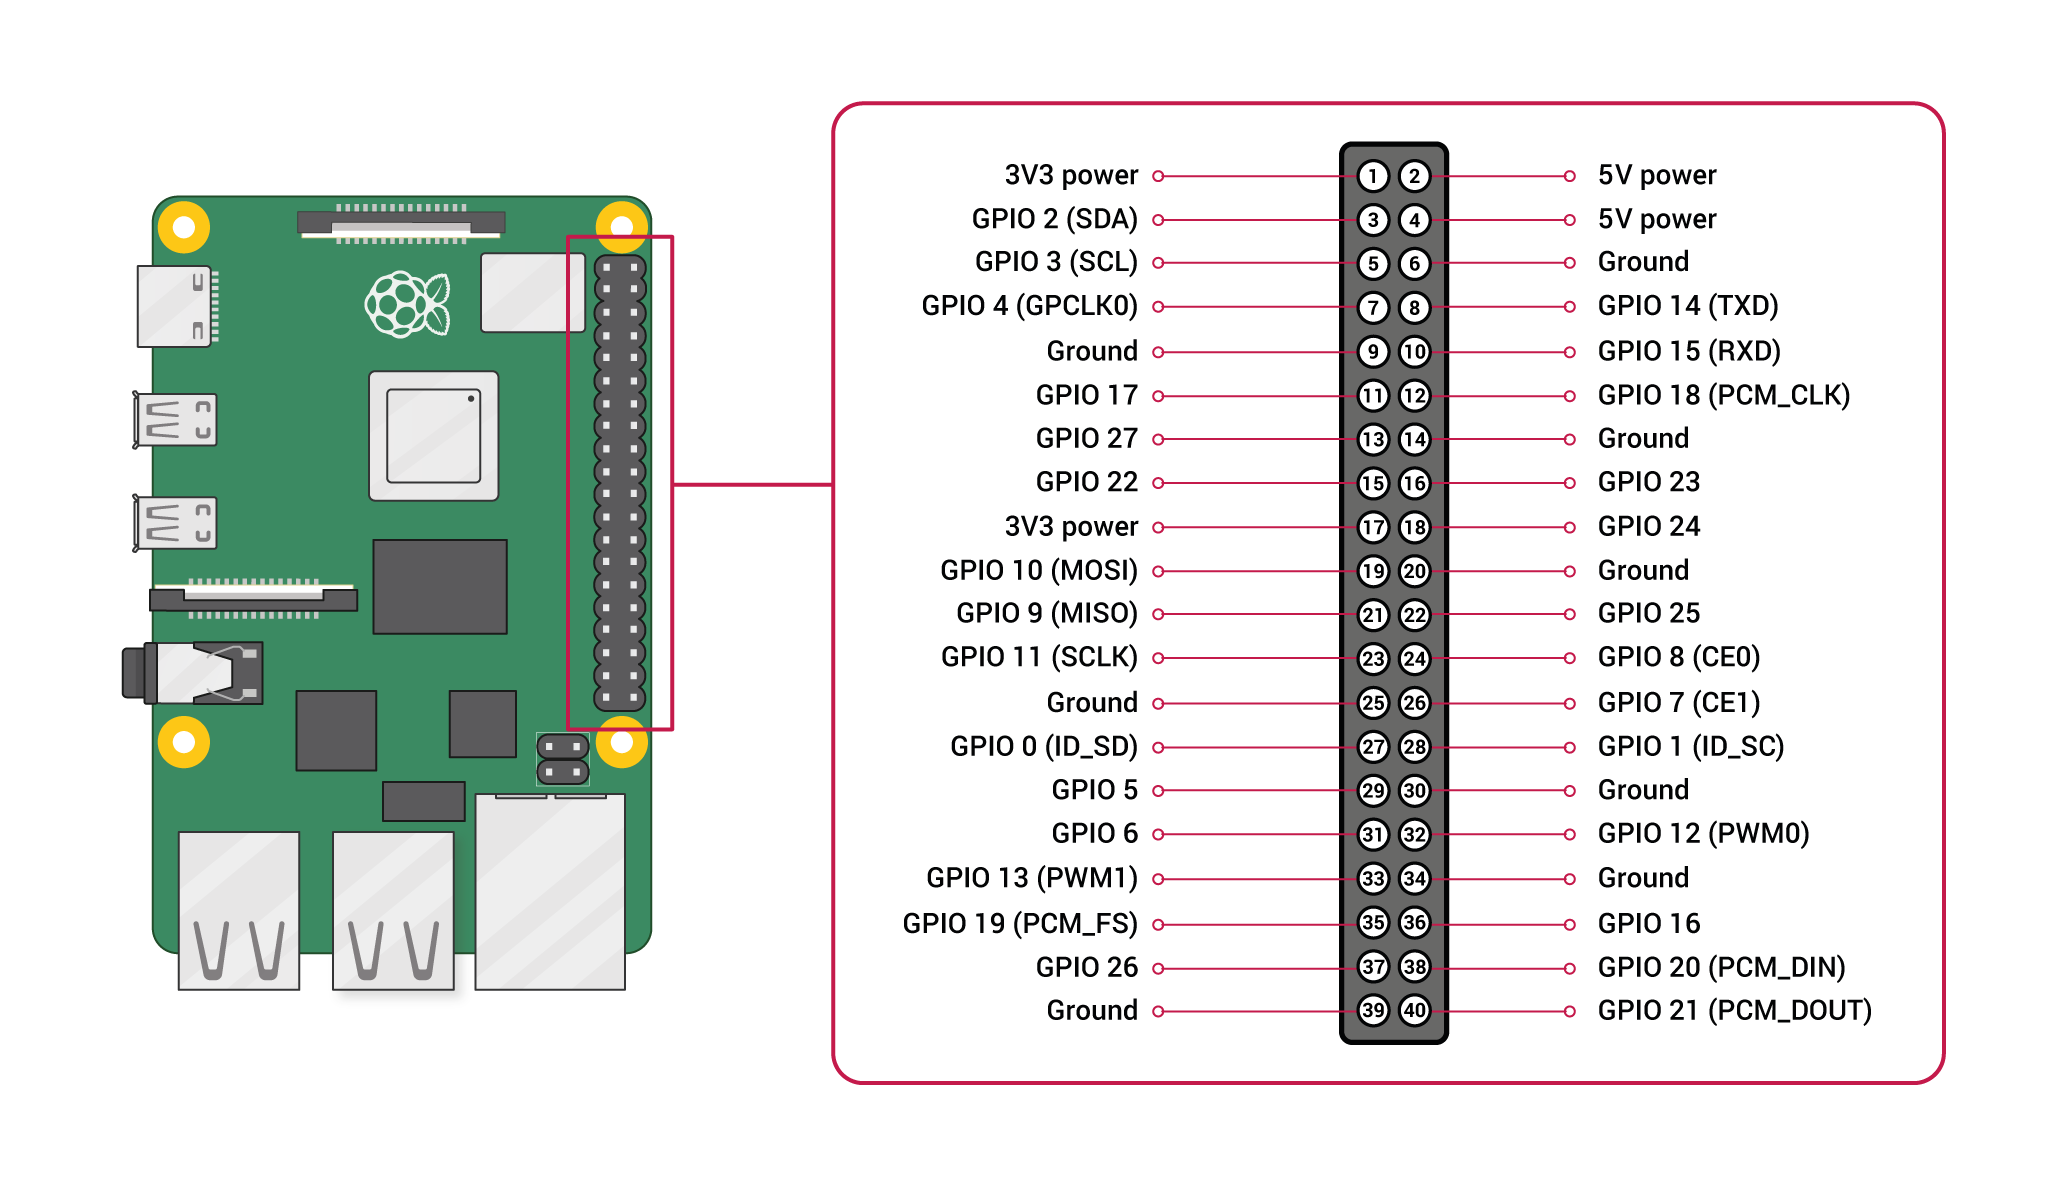
\includegraphics[width=8cm]{gambar/GPIO-Pinout-Diagram-2.png}
        \caption{Pinout Raspberry Pi 3B}
        \label{pinout}
  \end{figure}


  \section{NodeMCU}
  NodeMCU adalah mikrokontroler yang dilengkapi dengan modul wifi esp8266. 
  Secara fungsi NodeMCU mirip dengan Arduino, hanya saja NodeMCU sudah dilengkapi dengan wifi.

  \section{Thingsboard}
  Thingsboard merupakan salah satu IoT platform yang open source. 
  Fitur yang terdapat pada thingsboard dapat mempermudah penggguna dalam pengembangan produk, manajemen maupun \emph{scaling} produk. 
  Terdapat 9 menu pada halaman \emph{home}. 
    \begin{enumerate}
      \item HOME
      \item RULE CHAINS
      \item CUSTOMERS
      \item ASSETS
      \item DEVICES \\
      Pada menu ini, pengguna dapat mendaftarkan \emph{device} yang akan digunakan.
      \item ENTITY VIEWS
      \item WIDGETS LIBRARY
      \item DASHBOARDS
      Pada menu ini, pengguna dapat membuat tampilan \emph{dashboard} yang diinginkan
      \item AUDIT LOGS
    \end{enumerate}
  \section{MQTT}
  \section{HTTP}

  \chapter{Pembahasan}
  \section{Praktikum Minggu I}
    \subsection{Percobaan 1}
    Pada percobaan ini, praktikan membuat \emph{device} led pada Thingsboard.
    Setelah membuat \emph{device} maka akan mendapatkan akses token.
    Token tersebut berguna untuk mengakses \emph{device} tersebut.
    \subsection{Percobaan 2}
    Pada percobaan ini, praktikan menginstall \emph{board} NodeMCU dan beberapa \emph{library} yang akan digunakan.
    Terdapat 3 \emph{library} yang digunakan, antara lain:
    \begin{enumerate}
      \item ArduinoJSON
      \item PubSubClient
      \item ESP8266Wifi
    \end{enumerate}
    Source Code
    \begin{enumerate}
      \item \lstinputlisting[firstline=1,lastline=3]{../1/1.ino}
      Kode di atas digunakan untuk menambahkan \emph{library} yang akan digunakan. \\
      \item \lstinputlisting[firstline=5,lastline=12]{../1/1.ino}
      Kode di atas digunakan untuk mendefinisikan sebuah konstanta dan variable. \\
      \item \lstinputlisting[firstline=22,lastline=34]{../1/1.ino}
      Kode di atas digunakan untuk men-\emph{setup} pin, komunikasi serial, komunikasi MQTT, wifi yang akan digunakan. \\
      \item \lstinputlisting[firstline=36,lastline=44]{../1/1.ino}
      Kode di atas digunakan untuk menghubungkan kembali komunikasi mqtt jika terputus.
      \item \lstinputlisting[firstline=47,lastline=90]{../1/1.ino}
      Kode di atas digunakan untuk mendapatkan pesan dari sebuah topik pada komunikasi mqtt. 
      Pesan tersebut diolah, kemudian didapatkan nilai \emph{boolean}.
      Nilai \emph{boolean} tersebut digunakan untuk men-set gpio. \\
    \end{enumerate}
    
    \subsection{Percobaan 3}
    Pada percobaan ini, praktikan membuat dashboard yang digunakan untuk mengendalikan led.
    Dashboard tersebut berisi \emph{widget} yang telah diimport

    \subsection{Tugas}
    Terdapat 2 buah led yang dikendalikan melalui dashboard thingsboard. 
    Ketika tombol on pada dashboard thingsboard ditekan maka led pada rangkaian NodeMCU akan menyala, begitu sebaliknya.
    

  \section{Praktikum Minggu II}
  \subsection{Percobaan 1}
    Pada percobaan ini, praktikan membuat \emph{device} DHT11 pada Thingsboard.
    Setelah membuat \emph{device} maka akan mendapatkan akses token.
  \subsection{Percobaan 2}
    Percobaan ini bertujuan untuk mengirim data dari sensor DHT11 ke thingsboard menggunakan mqtt.
    Data yang dikirim adalah nilai dari \emph{Humidity} dan \emph{Temperature}.

  \subsection{Percobaan 3}
  \subsection{Tugas}
\section{Praktikum Minggu III}
    \subsection{Percobaan 1}
    Pada percobaan ini, praktikan mengirim data dari sensor jarak menggunakan mqtt ke platform thingsboard.
    Data tersebut dikirim 1 detik sekali. \\
    Source Code
    \begin{enumerate}
      \item \lstinputlisting[firstline=1,lastline=7,language=Python]{../3/3.py}
      Kode di atas digunakan untuk menambahkan \emph{library} yang akan digunakan. \\
      \item \lstinputlisting[firstline=10,lastline=15,language=Python]{../3/3.py}
      Kode di atas digunakan untuk melakukan konfigurasi pada pin yang akan digunakan. \\
      \item \lstinputlisting[firstline=17,lastline=26,language=Python]{../3/3.py}
      Kode di atas digunakan untuk men-\emph{setup} komunikasi MQTT dan komunikasi terhadap platform thingsboard. \\
      \item \lstinputlisting[firstline=33,lastline=51,language=Python]{../3/3.py}
      Kode di atas digunakan untuk mendapatkan data dari sensor jarak.
    \end{enumerate}
    \subsection{Percobaan 2}
    Pada percobaan ini, praktikan membuat \emph{device} HCSR04 pada Thingsboard.
    \emph{Device} tersebut berguna untuk menerima data yang berasal dari HCSR04. 
    Data yang terkirim dapat dilihat \emph{tab} \emph{LATEST TELEMETRY}.
    Data tersebut akan digunakan dalam membuat dashboard. \\
    Dashboard yang digunakan merupakan sebuah \emph{chart widget}.
    \emph{Chart widget} tersebut bertipe \emph{time series}.
    \subsection{Tugas}
    Percobaan ini bertujuan untuk mengambil data dari sensor DHT11 dan mengirimkannya ke Thingsboard. 
    Pengiriman data menggunakan protokol komunikasi mqtt. 
    Source Code
    \begin{enumerate}
      \item \lstinputlisting[firstline=37,lastline=39,language=Python]{../3/3_dht.py}
      Kode di atas digunakan untuk mendapatkan data \emph{humidity} dan \emph{temperature} sensor DHT11.
      Data tersebut kemudian dibulatkan.
      \item \lstinputlisting[firstline=45,lastline=45,language=Python]{../3/3_dht.py}
      Kode di atas digunakan untuk mengirim data ke Thingsboard.
      Data yang dikirim berbentuk JSON. \\
    \end{enumerate}
  \section{Praktikum IV}
  \subsection{Percobaan 1}
  Pada percobaan ini, praktikan menginstall beberapa \emph{library} antara lain :
  \begin{enumerate}
    \item Seeed Studio
    \item Thingsboard MQTT PubSubClient
  \end{enumerate}

  Source Code
    \begin{enumerate}
      \item \lstinputlisting[firstline=1,lastline=11,language=Python]{../4/4.py}
      Kode di atas digunakan untuk menambahkan \emph{library} yang akan digunakan. \\
      \item \lstinputlisting[firstline=14,lastline=21,language=Python]{../4/4.py}
      Kode di atas digunakan untuk melakukan konfigurasi format penulisan dan akses thingsboard. \\
      \item \lstinputlisting[firstline=26,lastline=47,language=Python]{../4/4.py}
      Kode di atas digunakan untuk mendapatkan data dari masing-masing sensor.
      Dalam percobaan ini hanya perangkat led dan servo yang digunakan. \\
      \item \lstinputlisting[firstline=50,lastline=61,language=Python]{../4/4.py}
      Kode di atas digunakan untuk menerima permintaan dari pengguna dan mengirim permintaan tersebut ke \emph{device}.
      Pengguna dapat mengirim perintah untuk menjalankan servo pada sudut tertentu dan mengontrol led. \\
    \end{enumerate}
  \subsection{Percobaan 2}
  Pada percobaan ini, praktikan membuat \emph{device} dan \emph{dashboard} pada Thingsboard.
  \emph{Dashboard} yang digunakan sudah disediakan oleh Seeed Studio.
  \subsection{Tugas}
  Percobaan ini merupakan gabungan dari percobaan 1 dan 2.
  Setelah \emph{dashboard} dibuat, pengguna dapat mengendalikan led dan servo melalui \emph{dashboard} tersebut.

  \section{Praktikum V}
  \subsection{Percobaan 1}
  \subsection{Percobaan 2}
  \subsection{Tugas}

  \section{Praktikum V}
  \subsection{Percobaan 1}
  \subsection{Percobaan 2}
  \subsection{Percobaan 3}
  \subsection{Tugas}
    
\end{document}